
\section{Introduction}
In modern financial markets, double auction is a standard process of buying and selling shares adopted by exchanges. From an economist's perspective, an auction can be considered as a price discovery process. A competitive equilibrium price is found through interactions among bidders where supply and demand are equal. The question of how the price reaches its equilibrium points, and how different players use their own information advantages to achieve a preferable price, has attracted attentions from various fields. \cite{Kyle1985} studies how market makers, insider traders and noise traders interact to form an equilibrium price in a continuous trading auction. \cite{Almgren2000} discusses how execution can be done optimally in a continuous trading phase under certain market impact assumptions. \cite{Avellaneda2008} derives an equilibrium price from the perspectives of a market maker to provide quotes in a continuous trading auction. This paper is in a similar vein, in which we discuss how price will reach its equilibrium price in a mixed auction market. By taking into account call auction, under different market impact assumptions, we derive the corresponding optimal liquidation strategy for a trader to unwind his position. We provide theoretical evidence that it is indeed cheaper to trade the call auction compared to the continuous auction. Specifically, we examine the market impact of trading in a market that operates under two auction models:

\begin{itemize}
  \item \textbf{Call auction} Buyers set a maximum price that they want to buy, and sellers set a minimum price that they want to sell. The orders will then be batched together and matched at a price set by the exchange.
  \item \textbf{Continuous auction} Orders are matched continuously based on time and price priority. Participants in the auction can choose to either queue their orders to wait for an opposing trade, or cross the book to match against other's orders.
\end{itemize}

We seek to reduce market impact and cost of trading by utilizing both auctions in our liquidation algorithm. The aim is to significantly reduce the cost of trading by exploiting liquidity from both, which can be achieved from answering the following questions:

\begin{itemize}
  \item What are the relevant factors that affect market impact during both auctions?
  \item How does the transition of market impact from a call auction into a continuous auction evolve?
  \item How can we optimize for a liquidation trading strategy, taken into account those factors?
\end{itemize}

In general, the challenge lies in the different mechanisms of the auctions, and the modelling of market impact during both thereof. By modelling the interaction between different participants in the market, namely between market makers and liquidity takers, we derive the mechanism of market impact under both auctions. From the mechanism, we optimize for a liquidation problem that results in on average 50\% reduction in transaction cost against the classical TWAP solution during continuous trading phase only.

It is not a coincidence that by incorporating call auction into the optimal liquidation problem, we can reduce cost significantly. Historically, the adoption of the call auctions has resulted in a substantial shift of daily trading activity, with the call auctions responsible for a significant proportion of the average daily trading volumes. (\cite{Madhavan2015}) found that the call auction in New York Stock Exchange (NYSE) accounts for roughly 10 percent of the average trade volume. (\cite{Bruno1999}) found similar phenomenon on the Paris Bourse, in which the opening auction accounts for about 10 percent of average daily trade value. (\cite{Carole2006}) has a similar conclusion regarding the Australian Stock Exchange (ASX).

A call auction can lower execution costs for participants and improve price discovery process, as suggested in (\cite{Pagano2003}). The reduction in trading costs, such as market impact and adverse selection costs, is achieved through several channels, including (\cite{Carole2006}):

\begin{itemize}
  \item Temporal consolidation of order flow and execution of orders at a single price (\cite{Economides1995}).
  \item Facilitation of price discovery process during times of market stress (\cite{Madhavan1992}).
\end{itemize}

Various studies have found that there are significant strategic trading activities during the call auctions. (\cite{Bruno1999}) suggests that the fluctuation in the indicative price during the call auction period maybe due to strategic trading. (\cite{Vives2001}) argues that large market makers may have incentives to trade during the opening call auction, to mitigate information leakage.

On the other hand, literature on optimal liquidation and market impact has rarely mentioned execution during call auctions, not to mention the mixed auction environment. One of the first study on optimal liquidation is (\cite{Ho1981}), in which an optimal trading curve is derived under certain assumptions on stochastic trade arrival and price process. (\cite{Almgren2000}) extends the model further by incorporating a trader's risk aversion factor when pricing for an optimal liquidation strategy. (\cite{Obizhaeva2013}) solves the problem under a different assumption: the impact of each trade recovers slowly instead of immediately. These works are derived for continuous auction. In terms of trading during a call auction, (\cite{Madhavan2015}) derives a optimal liquidation strategy for a specialist to set an equilibrium price under the assumptions of multiple traders with private information.

Works on optimal execution today focuses more on minimizing the impact of trading during the continuous trading phase, which ignores the fact that the opening auction is usually very liquid and the matched volume represents a significant portion of daily trading volume. For executing a big block order with significant volume, including call auctions are usually more preferable since the execution cost is lower, as shown in our analysis later. Specifically, based on our theoretical framework, we found that:

\begin{itemize}
  \item The call auction provides another venue to take liquidity from.
  \item Due to inventory management from the market maker, the transition period from the call auction will be characterized with a wide initial spread that will narrow over time. A mixed auction strategy takes into account this effect will reduce transition cost even further.
  \item There is an optimal liquidation strategy to execute trade during both the call auction and the continuous auction that results in better cost optimization than trading in the continuous auction only.
\end{itemize}

This paper is organized as follows: Section (\ref{sec:AnalyticalFramework}) will present the theoretical framework that we will use to characterize the call auction and optimize our trading strategy. Section (\ref{sec:EmpiricalAnalysis}) will perform empirical analysis based on the theoretical framework to examine their effects on the optimal liquidation strategy and its cost efficiency. Section (\ref{secConclusionAuction}) will conclude the paper with suggestions for further research.

\section{The Analytical Framework}\label{sec:AnalyticalFramework}

In order to derive an optimal liquidation strategy in a mixed auction market, we must first specify the auction mechanism for each session and how trading will impact the fair price of the market. We consider a market with two trading sessions in succession: a call auction session and a continuous trading session. The mechanism of each session, number of participants in each session and how their interaction affects the price of the underlying risky asset will be described, following by the market impact formula and the optimal liquidation strategy.

\subsection{Call auction mechanism and agents' behaviours}\label{subsec:AnalyticalFrameworkCallAuction}

In this section we will examine how different participants contribute to the price discovery process during the call auction. We assume the call auction is fully automated, and the matching mechanism is modelled after a Walrasian auction. Traders can submit and amend orders anytime during the call auction. Those orders are not matched immediately, and placed into the book as "crossed", that is, the highest buy price is higher than the lowest sell price in the book (see Table (\ref{itayoseTable1}) for an example book during the call auction). At the end of the auction period, the orders in the book are matched based on an equilibrium price calculated by the exchange. The equilibrium price is determined to maximize the volume traded in the call auction, and therefore has to satisfy the following requirements:

\begin{itemize}
  \item All buy/sell orders at prices higher/lower than the equilibrium price must be executed.
  \item At the execution price, the entire either buy or sell quantity must be matched.
\end{itemize}

Table (\ref{itayoseTable2}) gives an example of how a book can be "un-crossed" at the end of the call auctions. All the orders that are unmatched at the end of the call auction will be transferred to the continuous trading session. There is no specialist who can step in to modify the equilibrium price. This mechanism is adopted for the opening call auctions in Singapore Stock Exchange (SGX), Tokyo Stock Exchange (TSE) and Nasdaq Stock Market (NASDAQ). New York Stock Exchange (NYSE) is different, in which a specialist sets the equilibrium price that is not necessarily the same as the volume-maximizing Walrasian price.

\begin{table}[]
  \centering
  \begin{tabular}{c|c|c|c|c}
    \hline
    \textbf{Total Buy} & \textbf{Buy} & \textbf{Price} & \textbf{Sell} & \textbf{Total Sell} \\ \hline
                       &              & 56             & 4000          & 16100               \\ \hline
                       &              & 55             & 10000         & 12100               \\ \hline
    3000               & 3000         & 54             & 2000          & 2100                \\ \hline
    3100               & 100          & 53             & 100           & 100                 \\ \hline
    7100               & 4000         & 52             &               &                     \\ \hline
    10100              & 3000         & 53             &               &                     \\ \hline
  \end{tabular}

  \caption{A sample crossed orderbook during call auction. The orders will be matched at the equilibrium price of 54, which results in 2100 shares traded.}
  \label{itayoseTable1}
\end{table}


\begin{table}[]
  \centering
  \begin{tabular}{c|c|c|c}
    \hline
    \textbf{Buy} & \textbf{Price} & \textbf{Sell} & \textbf{Trade} \\ \hline
                 & 56             & 4000          &                \\ \hline
                 & 55             & 10000         &                \\ \hline
    900          & 54             &               & 2100           \\ \hline
    100          & 53             &               &                \\ \hline
    4000         & 52             &               &                \\ \hline
    3000         & 53             &               &                \\ \hline
  \end{tabular}
  \caption{A sample orderbook at the end of the call auction.}
  \label{itayoseTable2}
\end{table}

Inspired by the framework in (\cite{Madhavan2015}), we model the call auction as a two-stage game. Orders are submitted by all participants in first stage of the game, during the call auction period. In the second stage, the book is matched based on the Walrasian price described above. We assume that there are two types of participants:

\begin{itemize}
  \item Market markers are those with private information about the value of the asset. This information is not necessary from possessing some insider knowledge about the asset, but from having access to superior information regarding the order flow of the book, such as real-time trades and quotes provided by the exchange and better data processing capability.
  \item Liquidity traders are those without private information and simply want to execute their orders. We assume the demands of liquidity traders are exogenous, and they trade using market orders.
\end{itemize}

Unlike (\cite{Madhavan2015}), we do not assume that there is a specialist setting the equilibrium price, as most exchanges around the world has adopted automated call auction mechanism at the time of this writing. We also do not assume that there are informed traders with information advantage, but a market maker who holds private information and make the market instead. There are several reasons for this setup:
\begin{itemize}
  \item The model setup assumes that, in order to fully utilize the information advantage, the participant who holds it must have the ability to reprice his orders immediately after he receives a new signal. As we assume the private information is mainly from observing the order flow of the book, it means the participant is a high frequency trader (HFT), who can act immediately after each change in market order flow.
  \item There are evidences that a significant portion of high frequency trading during is for liquidity provision. (\cite{Menkveld2013}) studied the trading activity in Chi-X Europe, and found that a majority of high frequency trading activities is market making. Similarly, \cite{Bellia2017} found that there is a correlation between low-latency trading and the subsequent liquidity provision in the call auction in Tokyo Stock Exchange (TSE).
\end{itemize}

We further assume that there is a single market maker who makes the market for $K$ liquidity traders. This can be either a designated market maker obligated to provide liquidity for the market, or an external agent who wants to capture the liquidity premium of the call auction. The market maker is then assumed to have a negative exponential expected utility function of the form
\[
  u(W_e) = -e^{-\lambda W_e}
\]
where $W$ is the terminal wealth of the trader at the end of the call auction. The terminal wealth of the market maker is
\[
  W_e = p_0 (q + e_e) + (c_e - p_e q)
\]
The notions are
\begin{itemize}
  \item $\lambda>0$ is the risk aversion factor of the market maker.
  \item $p_0$ is the stock's fair price at the end of the call auction.
  \item $p_e$ is the stock's equilibrium price at the end of the call auction.
  \item $c_e$ is the initial cash position of the market maker.
  \item $e_e$ is the overnight position of the market maker.
  \item $q$ is number of shares purchased by the market maker at the end of the call auction.
\end{itemize}
To model the asset price at the end of the call auction, we assume that the asset value $p_0$ follows normal distribution with mean $\mu_e$ and precision (the inverse of the variance) $\zeta_e$ \footnote{While this means the stock may have negative price as time goes by, we can ignore this risk as we only need to account for one day of variance. Using an arithmetic stock price process instead of the classical logarihmic price process simplifies other calculation later in the study.}. The private information of market maker $\omega_e$ is then the normal variable
\[
  \omega_e \sim N(p_0, \frac{1}{\psi_e})
\]
The posterior distribution of the asset according to market maker's information set $\Omega_e$ is then normally distributed with mean
\[
  p_0=E[p_0|\Omega_e]=\mu_e \alpha + \omega_e(1 - \alpha)
\]
where
\[
  \alpha = \frac{\zeta_e}{\zeta_e+\psi_e}
\]
and variance
\[
  \sigma_e^2=var[v|\Omega_e]=\frac{1}{\zeta_e+\psi_e}
\]
Maximizing expected utility of the market maker, we have the amount of shares submitted
\begin{equation}\label{eqn:mm_eval_eqb}
  q(p) = a_e - b_e p
\end{equation}
where $a_e = \frac{p_0}{\lambda \sigma_e^2} - e_e$ and $b_e=\frac{1}{\lambda \sigma_e^2}$. We assume the $K$ liquidity traders will submit a total of $\sum_{i=0}^K x_i$ shares into the call auction to be matched, with negative values implying selling and vice versa. The total shares transacted at a given price $p$ is then
\[
  Q(p) = (p_0 - p) b_e + \sum_{i=0}^K x_i
\]
At equilibrium, we set $Q(p)$ to 0. This gives the Walrasian price as the matching price at the end of the call auction
\begin{equation}\label{markup_px_eqb}
  p_e = p_0 + \frac{\sum_{i=0}^K x_i}{b_e}
\end{equation}
The matching price is the fair price of the stock with a mark-up in proportion to the supply-demand imbalance in the market. The pricing function is plotted in Figure (\ref{fig:mm_pricing_auction}), which we will use to price our market impact of trading with the call auction in subsection (\ref{subsec:AnalyticalFrameworkTransitionPeriod}) after we examine the continuous trading phase in the next section.

\begin{figure}[h]
  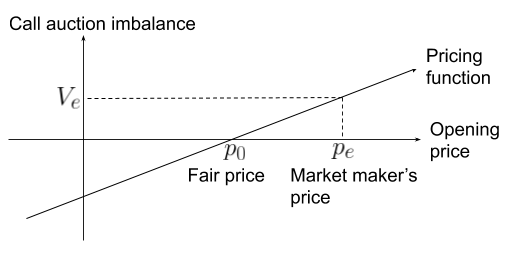
\includegraphics[width=\textwidth]{\OptimalAuctionPath/images/MMPricing}
  \caption{Pricing function of the market maker w.r.t call auction imbalance. If the imbalance is negative, implying that the sell demand is higher than buy demand, the market maker will price the opening price to be lower than his fair price, and vice versa. The slope of the pricing function is $\frac{1}{b_e}$ in Equation (\ref{markup_px_eqb}). $V_e$ is the imbalance at the end of the call auction, while $p_e$ is the opening price. }
  \label{fig:mm_pricing_auction}
\end{figure}

\subsection{Continuous auction mechanism and agents' behaviours}\label{subsec:AnalyticalFrameworkContinuousAuction}
During the continuous trading session, orders can be posted into the market at anytime during the session to be matched. If a buy order has a price that is higher than the current lowest offer in the book, it will be matched immediately, and vice versa for a sell order. Otherwise, it will be added into the book.

Similar to the call auction, we model the continuous auction as a multi-round two-stage game. At the beginning of each round, we pick randomly a liquidity trader to act as the counterparty of the market maker. In the first stage of the round, the market maker place limit orders in the book according to his risk tolerance and private information. In the second stage, the liquidity trader will place a market order based on his exogenous demand. This setup is slightly different from the call auction in which:
\begin{itemize}
  \item Unlike the call auction, only the market maker can submit limit orders during the first stage of the game. He has no knowledge of the liquidity trader's order, and only submit orders based on his own evaluation of the asset's value.
  \item The liquidity trader can only submit market orders during the final stage of the game, after the market maker has finished layering his orders in the book.
\end{itemize}
Under this mechanism, the market maker has a speed advantage with respect to the rest of the market, since he can evaluate the current fair pricing of the asset after each trade. After the reevaluation, he can modify his orders in the market to reflect the updated belief before any liquidity traders can place a new order. This grants the market maker distinct competitive advantage, in the sense that he can reprice his orders in the book before getting hit by any adverse selection event. This gives incentive to market makers to perform high frequency trading.

Similar to the call auction, we assume the market maker has private information about the asset from his superior analytical capability. Again, let assume the immediate asset value at the end of the continuous auction's round is a random variable $v_c$ normally distributed with mean $\mu_c$ and precision $\zeta_c$. The market maker deduces his own evaluation with a private signal
\[
  \omega_c \sim N(v_c, \frac{1}{\zeta_c})
\]
and forms a posterior belief on the asset value at the end of the round as a normal random variable with mean
\[
  v_c=\mu_c \alpha + \omega_c(1 - \alpha)
\]
where
\[
  \alpha = \frac{\zeta_c}{\zeta_c+\psi_c}
\]
and variance
\[
  \sigma_c^2=\frac{1}{\zeta_c+\psi_c}
\]

At the beginning of each round, the market maker has a position $e_c$ that he wants to liquidate. Maximizing the market maker's utility function, we have his order quantity function in the book:
\begin{equation}\label{eqn:mm_eval_cont}
  q_c(p) = a_c - b_c p_c
\end{equation}
where $a_c = \frac{v_c}{\lambda \sigma_c^2} - e_c$ and $b_c=\frac{1}{\lambda \sigma_c^2}$. Let assume the liquidity trader needs to transact $x_0$ shares. The average price he gets after submitting his market order is
\[
  p_{avg} = \frac{a_c-x_0}{b_c}=p_0 - \frac{1}{b_c} x_0
\]
where
\[
  p_0 = \frac{a_c}{b_c}
\]
is the best price quoted by the market maker. Note that the position is from the perspective of the market maker, that is, the higher number of shares the liquidity trader wants to buy, the higher markup price he will have to pay to transact immediately. In other words, the markup price that the liquidity trader receives is
\begin{equation}\label{eqn:markup_px_cont}
  p_{avg} = p_0 + \frac{1}{b_c} x_0
\end{equation}

Comparing Equation (\ref{markup_px_eqb}) and Equation (\ref{eqn:markup_px_cont}), we can see that, ceteris paribus, the instantaneous market impact of trading during the auction phase has a higher chance of getting offset by other liquidity traders in the market. On the other hand, during the continuous phase, the liquidity trader will always receive an adverse markup price implied in market maker's quotes. This is clearer once we examine the transition period immediate after market opening in the next subsection.

\subsection{Price discovery at market opening}\label{subsec:AnalyticalFrameworkTransitionPeriod}

There is empirical evidence that the transition period immediate after market opening is crucial in determining the effectiveness of the opening call auction (\cite{Pagano2013}). In this subsection, we analyze how the market maker, and consequently the spread, may behave during this period, and the subsequent effects on the liquidity trader. Recalling from Equation (\ref{markup_px_eqb}), the opening price is marked up proportional to the buy-sell imbalance at the end of call auction. Let
\[
  V_e = \sum_{i=0}^K x_i
\]
be the imbalance at the end of call auction. Based on the imbalance, the market maker will provide the liquidity necessary for the market to open at price
\[
  p_e = p_0 + \frac{V_e}{b_e}
\]
Without loss of generality, let $V_e$ be positive, implying that the market has more buy interests than sell interests. The market maker will sell $V_e$ shares at price $p_e$ higher than his estimated fair value of $p_0$, and has an unrealized gain of
\[
  G_e = (p_0 - p_e) * V_e
\]
To capitalize this gain after market opening, the market maker will need to make a spread. Continuing from the call auction's we have the pricing function of the market maker during this period:
\[
  q(p) = a_e - b_e p
\]
where $a_e = \frac{p_0}{\lambda \sigma_e^2} - V_e$ and $b_e=\frac{1}{\lambda \sigma_e^2}$, based on his signal when pricing the call auction. As $V_e$ is positive, this implies that the market maker is willing to sell at $p_e$. On the other hand, it is reasonable to assume that he will want to liquidate his position acquired from the opening call auction at $p_0$, his fair price of the asset at the end of the call auction. Therefore, the market maker will make a spread of $\frac{V_e}{b_e}$ immediately after call auction. The quotes of the market maker are illustrated in Figure (\ref{fig:mm_pricing_transition}).

\begin{figure}[h]
  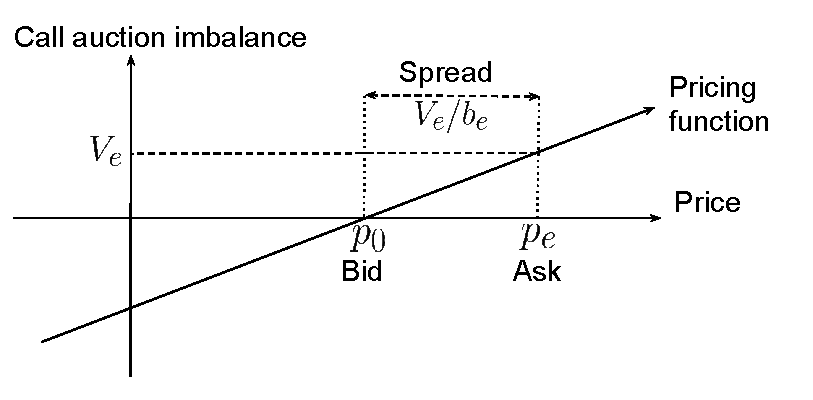
\includegraphics[width=\textwidth]{\OptimalAuctionPath/images/MMPricingTransition}
  \caption{Market maker's quotes immediately after opening w.r.t call auction imbalance. Upon market opening, the market maker will short $V_e$ shares at $p_e$. His evaluation of the asset's fair value is at $p_0$. However, due to his inventory, he will quote the ask side further away at $p_e$, and bid side at $p_0$. The bid-ask spread is then $\frac{V_e}{b_e}$, based on the market maker's pricing function (\ref{eqn:markup_px_cont}).}
  \label{fig:mm_pricing_transition}
\end{figure}

Interestingly, the bid-ask spread after market opens reveals the market maker's pricing in the call
auction, as we can calculate the implicit factor $b_e$ as
\begin{equation}\label{eqn:expected_spread}
  b_e = \frac{V_e}{\zeta_e}
\end{equation}
where
\begin{itemize}
  \item $V_e$ is the matching volume at the open of continuous trading session.
  \item $\zeta_e$ is the spread at the open of continuous trading session.
\end{itemize}

From the similarity of the pricing function during the call auction in Equation (\ref{markup_px_eqb}) and the continuous auction in Equation (\ref{eqn:markup_px_cont}), we can see that, ceteris paribus, it is advantageous to trade in both sessions to consume liquidity from both to lower his market impact. This will be clearer once we derive the optimal trading strategy in the next section. Moreover, as the call auction compresses the liquidity over a long period of time in one single price, there is usually a much larger quantity traded than an average market order during continuous auction. Consequently, the market marker will need to unwind the position acquired from the call auction over a transition period immediately after the matching. This will affect the pricing for the liquidity trader during this period, in addition to the normal pricing in the continuous session. Specifically, the liquidity trader will potentially face one of the following two scenarios during the call auction:

\begin{itemize}
  \item {\textbf{Scenario 1: The liquidity trader trades in the same direction as the market imbalance}
        As $V_e$, the buy-sell imbalance at the end of the call auction, is assumed to be positive, we have the liquidity trader wants to buy in this case. As a result, his block trade size of $B_0$ will push the opening ask up, from $p_e$ to
        \[
          p_{e+} =  p_0 + \frac{V_e + B_0}{b_e}
        \]
        As he is buying, this is equivalent to lifting the offer during the continuous phase. In this case, ceteris paribus, there is no difference between trading during the auction and trading during the continuous phase.

        \begin{figure}[h]
          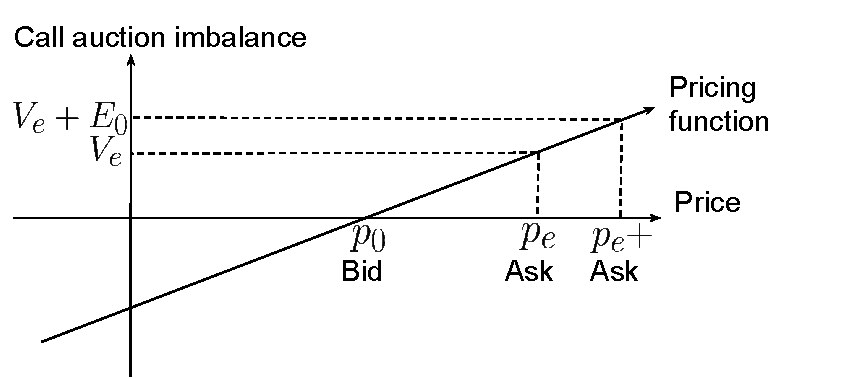
\includegraphics[width=\textwidth]{\OptimalAuctionPath/images/MMPricingTransitionSameDir}
          \caption{Bid-ask spread under Scenario 1, in which the liquidity trader trades in the same direction as the bid-ask imbalance. Consequently, he will push the ask price up, increase the cost of trading both in the call auction and the subsequent continuous phase.}
          \label{fig:mm_pricing_transition_s1}
        \end{figure}
        }
  \item {
        \textbf{Scenario 2: The liquidity trader trades against the market imbalance}
        In this case, the liquidity trader will sell to the market, similar to the market maker. Therefore, he is providing liquidity to the market, reducing the bid-ask spread immediately after market opening. Consequently, the opening price bid will improve from $p_e$ to
        \[
          p_{e-} = p_0 + \frac{V_e - B_0}{b_e}
        \]
        As he is selling, this is equivalent to placing his offer into the bid-ask spread during the continuous phase and getting filled immediately.
        \begin{figure}[h]
          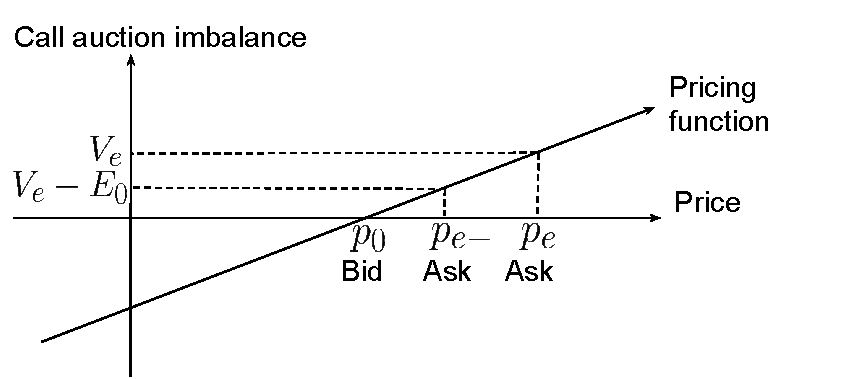
\includegraphics[width=\textwidth]{\OptimalAuctionPath/images/MMPricingTransitionDifferentDir}
          \caption{Bid-ask spread under Scenario 2, in which the liquidity trader trades against the bid-ask imbalance. Consequently, he will pull the opening ask price down, while leave the opening bid at $p_0$. As he is selling, there is no impact on his cost of trading after market opening.}
          \label{fig:mm_pricing_transition_s2}
        \end{figure}
        }
\end{itemize}
As the market maker is buying at the fair price of $p_0$ and selling at a discounted price $p_e$, it is reasonable to assume that he will get filled more on the bid side than the ask side. This allows the market maker to reduce his inventory over time, and therefore tighten the bid-ask spread. Depending on which scenario the liquidity trader fallse into, the market maker's behaviour may affect his cost of liquidation. Specifically, we have:

\begin{itemize}
  \item Under Scenario 1, trading in the call auction results in an ongoing penalty cost to the liquidity trader that will decay over time, as he will need to lift the offer to buy. Let the speed of liquidation of the market maker be $\rho$ and $V_t$ be the remaining position of the market maker acquired from the call auction in Scenario 1. Consequently, we have
        \[
          dV_t = -\rho V_t
        \]
        \[
          V_t[0]=(V_e + B_0)
        \]
        \begin{equation}\label{eqn:recovery_term_eqb}
          \Leftrightarrow V_t = (V_e + B_0) e^{-\rho t}
        \end{equation}
        where $B_0$ is the liquidity trader's block trade size during auction. The resulting spread due to our trading during the call auction at time $t$ will be
        \[
          \zeta_t = \frac{e^{-\rho t}}{b_e}  (V_e + B_0)
        \]
        Therefore, we would expect the spread to be wide initially, and slowly closing due to the inventory management effects from the market maker. This is in agreement with current empirical evidence that the bid-ask spread narrows shortly after market opens.
  \item Under Scenario 2, trading in the call auction has no "spillover" effect on the liquidity trader, as the liquidity trader will keep hitting the bid to sell while the market maker will try to improve the offer.
\end{itemize}

This "spillover" cost only incurs half of the time under Scenario 1, while under Scenario 2 there is no additional cost for the liquidity trader during the continuous phase. Therefore, the expected markup cost to the liquidity trader during this transition period is:

\begin{equation}\label{resilence_term}
  \zeta_t = \frac{e^{-\rho t}}{2 b_e}  (V_e + B_0)
\end{equation}
which we use in the next section to derive the optimal liquidation strategy for the liquidity trader.

\subsection{Optimal liquidation strategy in a mixed auction market}

Based on the behaviors of market makers in the previous subsections, we can derive the market impact of trading for the liquidity trader across the sessions. Let the fundamental price process $S_t$ at time $t$ be
\[
  S_t = S_0 + \int_0^t \sigma dZ_s
\]
that is, $S_t$ follows a classical arithmetic random walk without any drift. The actual price process $P_t$ is then the combination of the fundamental price process $S_t$ and a short term deviation process $D_t$ due to the market maker repricing his book, as described in Subsection (\ref{subsec:AnalyticalFrameworkCallAuction}) and (\ref{subsec:AnalyticalFrameworkContinuousAuction}):

\[
  P_t = S_t + D_t
\]

From Equation (\ref{markup_px_eqb}) and Equation (\ref{eqn:markup_px_cont}), we can add into $D_t$ a linear cost component proportional to the trading sizes under each session:
\begin{equation}\label{short_term_deviation}
  D_t = \alpha B_0 + E_t \beta
\end{equation}
where
\begin{itemize}
  \item $B_0$ is the block trade size at the end of the call auction
  \item $E_t$ is the continuous trading rate of the liquidity trader
  \item $\alpha$ and $\beta$ are the cost penalty factor for aggressing the book during the call auction and continuous auction, respectively. We have $\alpha=\frac{1}{b_e}$ and $\beta=\frac{1}{b_c}$ based on Equation (\ref{markup_px_eqb}) and Equation (\ref{eqn:markup_px_cont}), respectively.
\end{itemize}
Equation (\ref{short_term_deviation}) is similar to what has been described as the "temporary impact" term in in the pioneering works of (\cite{BertimasLo1999}) and (\cite{Almgren2000}). On the other hand, from Equation (\ref{resilence_term}), we have the expected spillover cost of trading during call auction to continuous phase is:
\[
  R_t = \frac{\alpha (B_0 + \bar{V_e}) e^{-\rho t}}{2}
\]

The short term deviation term $D_t$ is then
\[
  D_t = \underbrace{\alpha B_0 }_\text{Cost of the call auction} +
  \underbrace{\frac{\alpha (B_0 + \bar{V_e}) e^{-\rho t}}{2}}_\text{Spillover cost} +  \underbrace{\beta E_t}_\text{Cost of the continuous auction}
\]
and the execution cost is
\begin{equation}\label{eqn:cost_equation_all}
  C_t = \alpha B_0^2 + \int_0^t \frac{\alpha (B_0 + \bar{V_e}) e^{-\rho t}}{2} E_s ds + \int_0^t \beta E_s^2 ds
\end{equation}

Based on the execution cost equation, we can derive an optimal strategy for the liquidity trader. Let assume the liquidity trader wants to unwind a large position, and he has the option to execute his trades in both the call auction and the continuous auction. We have the following notations regarding his trading strategy:

\begin{itemize}
  \item $Q_t$ is the total number of shares of his portfolio at time t.
  \item $E_t$ is the continuous liquidation strategy during the continuous trading auction.
  \item $X_t=\int_0^t E_s ds$ is the number of total executed shares at time $t$.
  \item $B_0=Q_0 - \int_0^T E_s ds$ is the size of the block trade executed at the end of the opening call auction.
\end{itemize}

Based on the Proof (\ref{proof:optimal-strategy-mixed-auction}) in the Appendix, we have the optimal size of block trade in the call auction as:
\[
  B_0 = \frac{Q_0 F_{11} + V_e F_{12}}{F_2}
\]
where
\[
  F_{11} = 8 e^{T \rho} \beta \rho [\alpha - e^{T \rho} (\alpha - 4 \beta \rho)]
\]
\[
  F_{12} = (e^{T \rho}-1) \alpha [\alpha (2+T \rho) + e^{T \rho} (8 \beta \rho + \alpha (T \rho - 2 ))]
\]
\[
  \begin{split}
    F_2 = \alpha^2 (2 + T \rho) - 4 e^{T \rho} \alpha (\alpha + 2 \beta \rho)
    + e^{2 T \rho} [8 \beta \alpha \rho + 8 \beta (T \alpha + \beta) \rho^2 + \alpha^2 (2 - T \rho)]
  \end{split}
\]
The optimal trading strategy during continuous session is:
\[
  E_t = A - B_0 \frac{\alpha e^{-t \rho}}{4 \beta}
\]
\[
  X_t = A t - B_0 \frac{\alpha (1- e^{-t \rho})}{4 \beta \rho}
\]
where
\[
  A =   \frac{4 (Q_0 - B_0) + \frac{(1 - e^{-T \rho})}{\beta \rho} B_0 \alpha} {4 T}
\]
The optimal trading strategy during auction phase is a modification of a TWAP strategy with an exponentially decayed component to account for the spillover effect. This is expected as a TWAP is proven to be optimal for a strategy with the cost of aggressing the orderbook only in (\cite{Ho1981}). A sample optimal allocation between the auction's block trade and the continuous trading strategy's size is in Figure (\ref{fig:optimal_sizes}). The corresponding optimal liquidation rate curve of the strategy is plotted in Figure (\ref{fig:optimal_curve_strategy}).


\begin{figure}[h]
  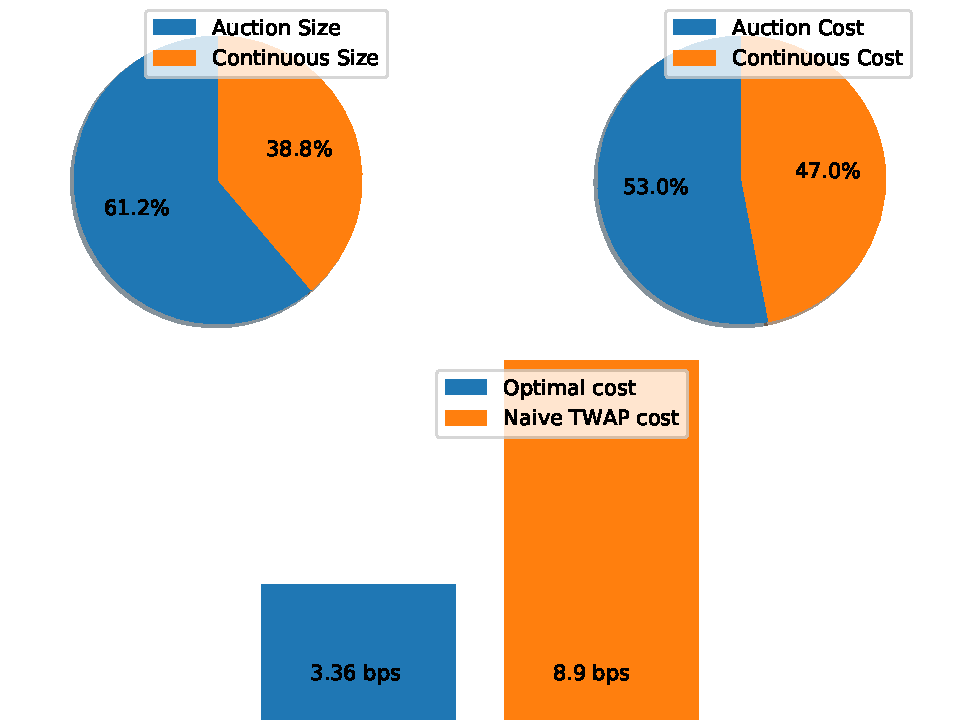
\includegraphics[width=\textwidth]{SampleTradeSize}
  \caption{Sample allocation between auction's block trade and the continuous trading strategy's size, using data from stock ACGL in October 2019, trading 5 percents of average trading volume of the first half of trading day. Compared to a pure TWAP trading stategy, the optimal stategy allocates 61.19 percents of the total position to be executed during the auction phase. The cost of trading in the auction phase accounts for 53.00 percents of the total cost of the strategy, while reducing 62.26 percents of total cost compared to a pure TWAP strategy, from 8.90 bps per share to 3.36 bps per share.}
  \label{fig:optimal_sizes}
\end{figure}



\begin{figure}[h]
  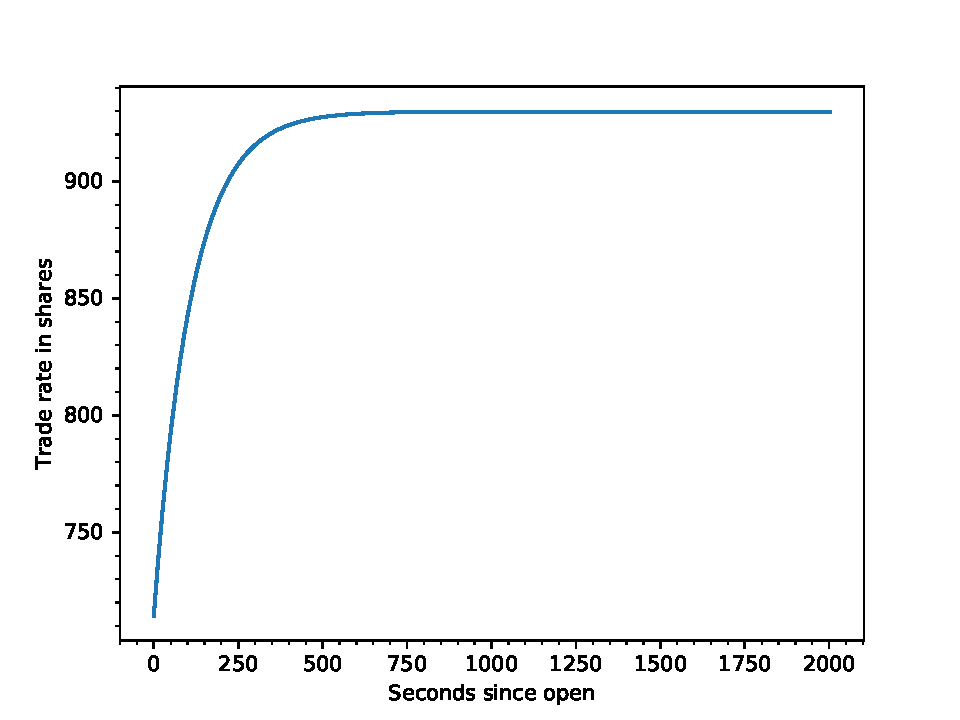
\includegraphics[width=\textwidth]{\OptimalAuctionPath/images/SampleTradeCurve}
  \caption{Sample optimal trading strategy's execution curve 30 minutes after market opens from auction phase. The shape of the optimal trading curve reflects the nature of the cost, in which the rate of execution is speed up over time as the market impact of the auction subsidizing and the spread narrowing.}
  \label{fig:optimal_curve_strategy}
\end{figure}

\subsection{Summary}

The main findings of this section can be summarized as follows:

\begin{itemize}
  \item The presence of informed trading from the market maker is required for the transition to continuous trading, as the market maker will provide the necessary liquidity to offset the buy-sell imbalance at the end of the call auction.
  \item The transition period from the call auction will be characterized with a wide initial spread narrowing over time due to inventory management from the market maker.
  \item Trading in the call auction lower the total execution cost compared to trading in continuous auction only, as the call auction provides an additional venue for liquidity consumption.
  \item There is an optimal liquidation strategy to execute trade during both the call auction and the continuous auction. The mixing ratio of the strategy is determined by the efficiency of each auction, in terms of immediate cost of aggressing the book and the speed of spread recovery after market opening.
\end{itemize}

Before moving to empirical analysis, it is imperative to address some stylized facts of our model. We assume that the liquidity traders are price takers who submit market orders to signify his intention to trade regardless of opening price, and the market maker will post limit orders to counter the imbalance. In most modern stock exchanges, all participants can post limit orders in the order book to be "crossed" during the opening match. Limit orders can also be modified or cancelled before the opening match, allowing participants to update their pricing. However, as long as the market maker in our model can place his trade after all the liquidity traders has submitted their orders, the pricing schedule based on the market imbalance still holds.

We also assume that there is only one market maker and only he or she trades with private information. In practice, there can be multiple agents trading with information. However, as long as the private information is derived from public data, that is, no insider trading, we can assume that all informed agent will have the same "signal" regarding the fair price of the stock, and are only different in their risk aversion factor. Therefore, we can assume that all informed agents are trading with same risk aversion factor, which are represented by the market maker in our model. The principal agent who provides liquidity in the call auction is assumed to be a market maker because, as shown in our model, he will need to make a spread in the continuous auction to capture the expected profit from his signal.

The source of private information is also a vital assumption in our model. We assume that the market maker derives his valuation from public information, which include, but not limited to, the following factors:

\begin{itemize}
  \item Public order flow, with or without identity.
  \item General market information, such as index futures movement before equity market opening.
  \item Price continuity from previous day's closing price. In absence of any fundamental news, it is reasonable to expect the opening price to be close to the previous day's closing price.
\end{itemize}

Another deviation is the inventory management effects of the market maker. In our model, there is market maker's inventory management effects on the spread due to the position acquired from the opening auction, but not in the continuous auction. While it would be more complete to account for the inventory management effects in both auctions, our empirical analysis suggests that the inventory management effects of the continuous auction is less prominent compared to the opening auction. Specifically, we observed that

\begin{itemize}
  \item There is little evidence that the bid-ask spread is changed following a trade except near the opening and closing auctions.
  \item The auction matching volume is usually much larger than a normal trade during continuous phase, accounted for a significant fraction of the daily trading volume.
\end{itemize}

Last but not least, although it is immaterial to our cost analysis, it is not obvious that the market maker will be profitable after placing his "stabilization" trade to counter the opening auction's imbalance. Even when his initial signal is correct up to the end of the opening auction, new information may come and he has to change his valuation of the stock before realize the signal from the call auction. This is evident in the high volatility immediately after market opening. However, the continuous book is only one of many execution venue for the market maker to realize his signal. For example, the market maker may attempt to "lock-in" his profit by hedging into the index futures immediately. He then can slowly unwind both legs of the hedge over the course of the day, resulting in a tightening spread over time.

With those caveats in mind, we can proceed to the empirical analysis of NASDAQ data to estimate the liquidation cost of trading in both auctions compared to only during the continuous auction.

\section{Application: optimal execution for a portfolio of stocks in mixed auction market}\label{sec:EmpiricalAnalysis}

In this section, we apply our model to the case of transaction cost analysis. We consider a liquidity trader who wants to transact in both the opening auction and the subsequent continuous trading auction of the NASDAQ stock exchange. While theoretically reasonable to expect significant reduction in execution cost compared to trading in continuous auction only, the uncertainty from the estimation of market impact factors may affect the efficiency of the optimal strategy. Consequently, the trader may want to assess this uncertainty if it is too large compared to the benefits of trading in both auctions. The trader's job is therefore to perform sensitivity analysis of his portfolio against different underlying factors. Specifically, the transaction cost analysis will need to answer the following questions:

\begin{itemize}
  \item What is the transaction cost of the portfolio for execution during the continuous auction only?
  \item How large the difference of the transaction cost when transact in both the call auction and the continuous auction compared to the continuous auction only?
  \item How accurate the estimation of the cost factors? How would this affect the accuracy of the execution cost estimation?
\end{itemize}

This section starts with the descriptive statistics of the stocks in the sample portfolio, along with the trading mechanism of the NASDAQ exchange. We then proceed to present the estimation method from public data, along with corresponding estimates and their variances. We perform sensitivity analysis with respect to three main cost factors:
\begin{itemize}
  \item Cost of trading in the opening auction.
  \item Cost of trading in the continuous auction.
  \item The recovery rate of market impact of auction trading in continuous phase.
\end{itemize}

We conclude the section with the summary of the sensitivity analysis, and the optimal course of action for the liquidity trader given his risk appetite.

\subsection{Data and market mechanism}

We use equity data from NASDAQ exchange in this study, which has operating mechanism resembling our theoretical model. Opening auction in NASDAQ is called \textbf{Opening Cross}. While similar to the general call auction described in our model, there are certain subtle difference between our model and the NASDAQ's Opening Cross:
\begin{itemize}
  \item Before the opening bell at 9:30 EST, NASDAQ allows investors to submit orders to two different books: a continuous book and an opening cross book. Orders submitted to the continuous book will be matched immediately and the matching information will be visible in the market data feed. Orders submitted to the opening cross book will be withheld to be matched later and are not visible in the market data feed.
  \item At 9:30 EST, the opening cross book and the continuous book will be merged together to form a single book, and a Opening Cross price will be calculated based on the following three rules, similar to our Walrasian matching rule:
        \begin{itemize}
          \item Maximize the number of shares executed.
          \item Minimize the imbalance of Cross orders.
          \item Minimize the distance from the Nasdaq inside bid-ask midpoint.
        \end{itemize}
        Matched orders and total matching quantity from the Opening Cross will then be disseminated in the market data feed. Market is considered to be in the continuous trading phase at this point of time.
\end{itemize}

While the presence of the continuous book during the call auction period deviates from our assumption, it makes little difference in practice due to limited volume transacted during this period. On the other hand, the hidden nature of the Opening Cross orders mean that we cannot directly derive the cost of aggressing the book during the call auction. However, based on the arguments in subsection (\ref{subsec:AnalyticalFrameworkTransitionPeriod}), we can infer the cost of trading during the call auction from the spread and matching volume immediate upon market opening.

The continuous auction in the NASDAQ exchange, on the other hand, is similar to our model.

Our data is captured directly from NASDAQ's ITCH-TotalView market data feed, provided by the National University of Singapore. The data contains all the add, modification, trade and delete for each order submitted to the continuous book, with fields indicating whether it is a buy or sell order. The data also contains the matching quantity and the Nasdaq Official Opening Price (NOOP) for each stock. Given the dataset of 3500 NASDAQ-listed stocks, we pick $200$ random stocks with the following constraints:
\begin{itemize}
  \item Since we do not account for the value of the queue priority in our market maker's modelling, we avoid selecting stocks with tick size higher than 10 basis points in our sample.
  \item We avoid low liquidity stock by selecting ones higher than 10M daily traded notional, which is roughly the first quartile of our sample.
\end{itemize}

Given those constraints, we use 1 week of data, from 01/10/2019 to 07/10/2019, in our empirical analysis. Since we only account for the market impact of the opening auction in our analysis, we use the data from 9:30 AM to 12:30 AM in our derivation. Due to the limited number of observations per stock, with only one opening auction a day, we group stocks by their relative tick sizes and trading volume to improve the accuracy of the estimations. As shown in subsequent analysis, those metrics capture the variance in our cost factors. The descriptive statistics of the data is in Table (\ref{tbl:stock_desc}). From the statistics, we can see that the sample represents a reasonable range of stocks in terms of traded volume and tick size.

\begin{table}
\centering
\caption{Summary statistics for each group of stocks based on daily volatility as percentage of average price. The diverse range of traded notional and tick size indicates that the sample includes stocks from various regimes in the population. The standard deviation is in the brackets.
}
\label{tbl:stock_desc}
\begin{tabular}{lrll}
\toprule
Volatility (\%/Px) &  Count & Volume (million \$/day) &   Tick (bps) \\
\midrule
           $<0.50$ &     32 &             3.87 (0.34) &  1.64 (0.55) \\
           $<1.00$ &     43 &             3.77 (0.38) &  0.97 (0.43) \\
           $<1.50$ &     34 &             3.90 (0.39) &  0.78 (0.47) \\
        $\geq 1.5$ &     41 &             3.91 (0.40) &  0.45 (0.38) \\
\bottomrule
\end{tabular}
\end{table}



\subsection{Estimation method}
In order to estimate the cost of trading, we need to estimate three factors:

\begin{itemize}
  \item The temporary book aggressing cost factor $\alpha$ before market opening in Equation (\ref{eqn:mm_eval_eqb})
  \item The temporary book aggressing cost factor $\beta$ during the continuous phase in Equation (\ref{eqn:mm_eval_cont})
  \item The spread recovery factor $\rho$ post opening auction in Equation (\ref{eqn:recovery_term_eqb})
\end{itemize}

In the following, we describe how those factors can be estimated from market data.

\subsubsection{Estimation of opening auction's cost factor $\alpha$}

As mentioned, NASDAQ does not publish order imbalance before market opening, but we can derive the cost factor $\alpha$ from the matching quantity and the opening bid-ask spread. Recall from Subsection (\ref{subsec:AnalyticalFrameworkTransitionPeriod}) that the market maker will be incentivized to provide the offseting liquidity $V_e$ for market to open, with price sensitivity coefficient $b_e$. The market maker will then need to make a spread of $\zeta_e$ to realize his expected profit from $V_e$. Assuming his price sensitivity coefficient $b_e$ does not change after market opening, we can estimate $b_e$ based on Equation (\ref{eqn:expected_spread}) as
\[
  \hat{b_e} = \frac{\bar{V_e}}{\bar{\zeta_e}}
\]
where
\begin{itemize}
  \item $\bar{V_e}$ is the average matching volume at the open.
  \item $\bar{\zeta_e}$ is the average spread at the open.
\end{itemize}

The estimation of cost factor $\alpha$ will then be
\[
  \hat{\alpha} = \frac{1}{\hat{b_e}}  = \frac{\bar{\zeta_e}}{\bar{V_e}}
\]

It should be noted that both $V_e$ and $\zeta_e$ are random variables, hence makes the measurement of the cost factor $\alpha$ follow a ratio distribution. Ratio distribution often is heavy-tailed and has high variance. For example, assuming that $V_e$ and $\zeta_e$ follow independent normal distribution with zero means, then $\alpha$ will follows Cauchy distribution, with both its expected value and variance undefined (\cite{Geary1930}). In reality, we expect $V_e$ and $\zeta_e$ to be both correlated and noncentral, making the exact distribution of $\alpha$ even more complicated. To mediate this, we use the log transformation of the ratio in our subsequent analysis. The rationale, according to (\cite{Katz1978}), is as follows:

Let assume $V_e$ and $\zeta_e$ to be correlated noncentral normal random variables. The cost ratio $\alpha$ then can be expressed as:
\[ \alpha \sim \frac{\mu_{\zeta_e} + \mathbb{N}(0, \sigma_{\zeta_e}^2 )}{\mu_{V_e} + \mathbb{N}(0, \sigma_{V_e}^2 )}
  = \frac{\mu_{\zeta_e} + \zeta_e}{\mu_{V_e} + V_e}
  = \frac{\mu_{\zeta_e}}{\mu_{V_e}}\frac{1+ \frac{\zeta_e}{\mu_{\zeta_e}}}{1+ \frac{V_e}{\mu_{V_e}}}
\]

Take logs to get
\[\log(\alpha) = \log \left(\frac{\mu_{\zeta_e}}{\mu_{V_e}} \right)
  + \log \left( 1+ \frac{\zeta_e}{\mu_{\zeta_e}} \right)
  - \log \left( 1+ \frac{V_e}{\mu_{V_e}} \right)
\]
Since $\log(1+\delta) = \delta - \frac{\delta^2}{2} + \frac{\delta^3}{3} + \dots $
then asymptotically
\[ \log(\alpha) \approx \log \left(\frac{\mu_{\zeta_e}}{\mu_{V_e}} \right)+ \frac{\zeta_e}{\mu_{\zeta_e}}  -
  \frac{V_e}{\mu_{V_e}}
  \sim \log \left(\frac{\mu_{\zeta_e}}{\mu_{V_e}} \right) + \mathbb{N} \left( 0, \frac{\sigma_{\zeta_e}^2}{\mu_{\zeta_e}^2} + \frac{\sigma_{V_e}^2}{\mu_{V_e}^2} \right)
\]

In other words, the log transformation allows us to consider the cost factor $\alpha$ approximately a Gaussian distributed random variable.

\subsubsection{Estimation of continuous auction's cost factor $\beta$}

Equation (\ref{eqn:markup_px_cont}) allows us to estimate cost factor $\beta$ directly from the liquidity posted in the book, with a slight adjustment. Since Equation (\ref{eqn:markup_px_cont}) is in terms of average price, we need to convert the price of the book to average price from the best bid-offer level, as illustrated in Table (\ref{tbl:bookAvgPxConversion}). Given the cumulative sum quantity as the independent variable $X$ and the average price as dependent variable $Y$, we have the $\beta$ estimate in a linear regression equation

\[
  Y_t = const + \beta * X_t + e_t
\]

One caveat is the period of observation for the regression. Given the discussion in Subsection (\ref{subsec:AnalyticalFrameworkTransitionPeriod}), we would want to avoid the transition period immediately after the opening. To identify this period, we perform two-sample t-test on consecutive 5-minute bin of data to determine if the average spread has stabilize. Specifically, given $\zeta_t$ as the average spread of the current bin and $\zeta_{t+1}$ as the average spread of the next 5-minute bin, the null hypothesis is:
\[
  H_0: \zeta_t = \zeta_{t+1}
\]
where the sample statistics of the spread mean is calculated as
\[
  \bar{\zeta_t} = \frac{\sum_{i=1}^N  \sum_{j=1}^5 \zeta_{ij}}{N*5}
\]
where $N$ is the number of days in our sample, and we measure the spread $\zeta_{ij}$ every 1 minute in each of the 5-minute bin. When we find the first 5-minute bin that we cannot reject the null hypothesis at $5 \%$ confidence level, we use the data in the bin as data for the regression. The sample statistics for $X$ and $Y$ is estimated similarly to the spread mean, where we bootstrap the average of 1-minute interval spread and cumulative sum quantity of the bin as sample data point. Furthermore, we use the data in the identified transition period to measure the recovery speed of the spread in the next subsection.

\begin{table}[h]
  \centering
  \begin{tabular}{c|c|c|c|l}
    \hline
    \textbf{Buy} & \textbf{Price} & \textbf{Sell} & \textbf{Sum} & \multicolumn{1}{c}{\textbf{Average Price}} \\ \hline
                 & 56             & 4000          & 14000        & 55.286                                     \\ \hline
                 & 55             & 10000         & 10000        & 55                                         \\ \hline
    900          & 54             &               & 900          & 54                                         \\ \hline
    100          & 53             &               & 1000         & 53.9                                       \\ \hline
    4000         & 52             &               & 5000         & 52.317                                     \\ \hline
  \end{tabular}
  \caption{A sample orderbook with average price calculated for each level. For example, the average price of the offer level 56 is $(55*10000+56*4000)/14000 = 55.286$}.
  \label{tbl:bookAvgPxConversion}
\end{table}

\subsubsection{Estimation of spread recovery rate $\rho$}

Given the transition period, we measure the average spread on a 1-minute interval:
\[
  \bar{\zeta_j} = \frac{\sum_{i=1}^N p_i}{N}
\]
where $j$ is the index of 1-minute interval, and $N$ is number of days in our dataset. From the time series $p_j$ we can perform an exponential linear regression to estimate $\rho$. We consider the following exponential model:
\[
  y = \theta e^{-\rho t}
\]
where the independent variable $t$ is number of seconds since market opening, and the dependent variable $y$ represented the average spread $\bar{\zeta_j}$.

\subsubsection{Data binning by volatility group}

While the estimation method is straightforward, there is one observation of each factor per stock per day, and our data span only 1 week of trading. Consequently, the estimates for each stock may not be representative of the cost factors' expected values. To improve the accuracy of the estimates, we group the data by each stock's daily volatility, normalized as percentage of its average price. The correlation between volatility and $\alpha$, $\beta$ and $\rho$ are $28\%$, $48\%$ and $24\%$, respectively. From the correlation, we hypothesize that the stocks' parameters within the same volatility bin will have similar distribution. Formally, let $F_\alpha$, $F_\beta$ and $F_\rho$ be the log distribution of $\alpha$, $\beta$ and $\rho$, respectively:
\[
  log \alpha \sim F_\alpha(\mu_\alpha,\sigma_\alpha|v)
\]
\[
  log \beta \sim F_\beta(\mu_\beta,\sigma_\beta|v)
\]
\[
  log \rho \sim F_\rho(\mu_\rho,\sigma_\rho|v)
\]
where $(\mu_\alpha,\sigma_\alpha)$, $(\mu_\beta,\sigma_\beta)$ and $(\mu_\rho,\sigma_\rho)$ are the means and standard deviations of the log of cost factors $\alpha$, $\beta$ and $\rho$ per volatility group $v$, respectively. The ratios are expected to be all positive and skewed towards zero, so we use log-transformation to make the sample more symmetric. Let $log \alpha*$, $log \beta*$ and $log \rho*$ be the sample mean per stock:
\[
  log \alpha* = \sum_{i=1}^m \alpha_i/m
\]
\[
  log \beta* = \sum_{i=1}^m \beta_i/m
\]
\[
  log \rho* = \sum_{i=1}^m \rho_i/m
\]
where $m$ is number of observations per stock. Based on the Central Limit Theorem, we have $log \alpha*$, $log \beta*$ and $log \rho*$ converge to normal distribution with means approximating expected values of cost factors per volatility group. We test the convergence using the Jarque–Bera test (\cite{JarqueBera1980}), reported along with the log estimates in the subsequent result summary.

\subsection{Transaction cost summary}

Based on the cost factor estimates per volatility group, table (\ref{tbl:param_estimates}) presents the estimates of the model for the group of stock based on daily volatility in our sample. In general, the estimates of cost factors per volatility group follows normal distribution with $5\%$ significance level. Therefore, we can assume that the estimates are representative of the expected cost factors per group.

The estimates in each group are positive and within a reasonable range to each other. This suggests that the estimation methods are robust to the choice of instruments. We also observe that:
\begin{itemize}
  \item The estimates of $log \alpha$ and $log \beta$ are in similar range. This suggests that our estimation of the auction cost factor from spread and auction matching quantity concurs with the cost implied in the liquidity posted in the continuous trading book. In other words, we expect the market maker to have consistent estimation of fair values across trading sessions, so $\alpha$ and $\beta$ should have similar values across volatility groups.
  \item The estimates of $log \rho$ are similar across volatility groups. This suggests that the recovery rate of the market impact during the auction matching is consistent across stocks and volatility bands.
\end{itemize}

\begin{table}
\centering
\caption{The average log of parameters per volatility group of the . The standard deviation is in the brackets. (**) indicates significant at 10\%, and (*) indicates significant at 5\%. In general, the sample means in each group converge to normal distribution, so we can assume that the sample means approximate expected values of the parameters per group.
}
\label{tbl:param_estimates}
\begin{tabular}{llllll}
\toprule
Volatility (\%/Px) & $log \alpha\ (bps/shr)$ & $log \beta\ (bps/shr)$ &    $log \rho$  &      $log V_e$  &     $log Q_0$  \\
\midrule
           $<0.50$ &          -6.10 (1.24)** &           -5.23 (1.07) &  4.27 (0.87)** &  10.41 (0.80)** &  7.32 (1.09)** \\
           $<1.00$ &          -4.92 (1.26)** &         -4.22 (0.88)** &  3.81 (0.84)** &   9.26 (1.34)** &  6.45 (1.18)** \\
           $<1.50$ &          -4.64 (1.09)** &         -3.62 (0.65)** &  3.80 (0.80)** &   8.63 (1.29)** &  6.28 (0.96)** \\
       $\geq 1.50$ &          -4.26 (1.25)** &         -3.17 (0.66)** &  4.39 (0.78)** &   8.50 (1.05)** &  6.02 (0.94)** \\
\bottomrule
\end{tabular}
\end{table}



We then proceed to calculate the execution cost of each group using the following cost measures:
\begin{itemize}
  \item Square-root cost ($C_1$): the standard method of market impact is the square-root formula
        \[
          C_1 = c \sigma \sqrt{\frac{n}{v}}
        \]
        where $C_1$ is the price change from executing a trade for $n$ shares, with market volatility $\sigma$, average daily volume $v$ and some constant $c$ (\cite{Toth2011}). We use this as a benchmark to our cost formula to ensure that our estimates are reasonable. Constant $c$ is set to one in our estimates. Note that the square-root cost only applies to cost of trading during continuous auction.
  \item TWAP cost ($C_2$): the total cost of executing a TWAP strategy during continuous trading session. The formula is:
        \[
          C_2 = \frac{Q_0 (2 Q_0 T \beta + \frac{1-e^{-T \rho} T V_e \alpha}{\rho})}{2 T^2}
        \]
  \item Optimal cost ($C_3$): the total cost of executing the optimal strategy in both the opening auction and the continuous session. The formula is:
        \[
          C_3 = B_0^3 \alpha + A^2 T \beta + \frac{A (1-e^{-T \rho}) V_e \alpha}{2 \rho} - \frac{B_0 e^{-T \rho} (B_0 + 2 V_e) \alpha^2 \sinh(T \rho)}{16 \beta \rho}
        \]
        where
        \[
          A =   \frac{4 (Q_0 - B_0) + \frac{(1 - e^{-T \rho})}{\beta \rho} B_0 \alpha} {4 T}
        \]
  \item Auction optimal cost ($C_4$): the cost of executing the optimal strategy in the opening auction. The formula is:
        \[
          C_4 = B_0^2 \alpha
        \]
  \item Continous optimal cost ($C_5$): the cost of executing the optimal strategy in the continuous session. The formula is:
        \[
          C_5 = C_3 - C4
        \]
  \item Optimal cost ratio ($C_6$): the ratio of the difference between cost of TWAP and the optimal strategy. The formula is:
        \[
          C_6 = \frac{C_2 - C3}{C_2}
        \]
\end{itemize}

The results are reported in Table (\ref{tbl:cost_report}). We can observe that:
\begin{itemize}
  \item The square-root law cost ($C_1$), the TWAP strategy's cost ($C_2$) and the optimal strategy's cost are on similar scale. This suggests our cost measures concurs with the square-root law of market impact. We can see that $C_2$ increases proportionally with the square-root cost, as the volatility increases. This suggests the more volatile a stock is, the higher its cost of aggressing the book.
  \item The difference between the square-root law cost ($C_1$) and the TWAP strategy's cost ($C_2$) widens significantly as volatility increases, even with constant $c$ in the square-root law adjusted. This implies that there is an additional component in the square-root law cost that is not captured in our formula. We hypothesizes that this is the permanent impact that moves the fundamental price up as we buy and down as we sell (See, for example, \cite{Kyle1985}). However, as shown in (\cite{Almgren2000}), this component is not optimizable.
  \item The improvement is significant across the volatility groups. This makes sense as the opening auction's pricing is similar to the continuous auction's pricing. Therefore, the opening auction provides an alternative venue to take liquidity from. By balancing his trades across two auctions, the liquidity trader can get cheaper pricing for his trades. 
  \item The optimal cost does not increase as much as the TWAP cost when volatility increases. Examining the auction proportion of the optimal cost, we can see the reason: the optimal strategy allocates the rising cost to the auction trade. The cost of trading in auction is consistently lower than continuous trading phase in (\ref{tbl:param_estimates}). Therefore, by allocate more shares to be execute in the auction, the optimal strategy lowers the rate of increase in cost compared to the TWAP strategy. The continuous portion of the optimal cost stays almost constant across volatility groups.
\end{itemize}

From those observations, we can see that the optimal strategy does not only lower the cost of trading compared to the TWAP strategy, but also help stablize cost among different volatility regimes. Therefore, the liquidity trader can achieve better control of his cost, as the optimal strategy is balanced against volatility.

\begin{table}
\centering
\caption{The average of cost measures grouped by tick size. Cost measures $C_1$ to $C_5$ are in bps per shares, while $C_6$ is in percentage points. The standard deviation is in the brackets.
}
\label{tbl:cost_report}
\begin{tabular}{lllllll}
\toprule
Volatility (\%/Px) &  $C_1$ & $C_2$ & $C_3$ & $C_4$ & $C_5$ &  $C_6$ \\
\midrule
           $<0.50$ &  11.18 &  5.88 &  2.35 &  1.39 &  0.97 &  59.94 \\
           $<1.00$ &  22.36 &  8.20 &  3.43 &  1.96 &  1.47 &  58.15 \\
           $<1.50$ &  33.54 &  7.50 &  3.05 &  1.77 &  1.27 &  59.38 \\
       $\geq 1.50$ &  44.72 &  9.67 &  3.45 &  2.20 &  1.26 &  64.29 \\
\bottomrule
\end{tabular}
\end{table}



\section{Conclusion}\label{secConclusionAuction}
We shows that when the cost of trading in the call auction is comparable to the continuous trading phase, our strategy yields significant cost savings. Subsequent research on different forms of market impact under both auctions, and extending to multi-phase auction market, can be conducted in the future to yield more interesting findings.
